\section{Ergebnisse / Evaluation}
%%%%%%%
% http://www.caps.in.tum.de/himmuc/
% Datenerhebenung (+ auf himmuc!) -> Max
% Skalierungs bzgl anzahl an nodes
% Vergleich OpenMP und mehrere MPI pro Node -> Tobi
% Overhead durch Balancer -> Florian
% Overhead durch MPI / Websocket / DrawTiles (konstant)
% Vergleich SIMD / Rohcode -> Niels

% Nutzbarkeit/ HCI -> Max
% vergleich x86 -> Max
% \subsection{Performanzerhöhung alternative Parallelisierungsmechanismen}

\subsection{Datenerhebung}
% Max
% Datenerhebung auf himmuc cluster
% Messen der Timings im backend (Wie kommen die Daten im frontend zu stande?)
% Auswahl der repräsentativen Punkte
% Grobes Intro zu der folgenden Evaluation
Die in den folgenden Abschnitten ausgewerteten Rechenzeiten für die Komponenten des Back- und
Frontends wurden in den entsprechenden Teilanwendungen in \( \mu s \) unter Verwendung der jeweiligen
Systembibliotheken (\verb|std::chrono|\footnote{\url{https://en.cppreference.com/w/cpp/chrono}} in \verb|C++| und \verb|Performance API|\footnote{\url{https://developer.mozilla.org/en-US/docs/Web/API/Performance}} in \verb|node.js|) gemessen.
Dabei stellt das so modifizierte Backend eine Erweiterung dar,
welche die gemessenen Zeiten zusätzlich in der Antwort der Regionsdaten an das Frontend
versendet. Dort werden diese aggregiert, mit den Zeiten des Frontend verknüpft und ausgegeben.

Um die Performance der folgenden Algorithmen auf der Mandelbrotmenge zu evaluieren,
müssen Regionen einzeln ausgewählt und die Performanz ihrer Berechnung verglichen werden.
Dafür haben wir die Mandelbrotmenge in drei Klassen unterteilt: Regionen in, am Rand und außerhalb
der Menge. Diese Aufteilung ist so gewählt, dass sich die Anzahl Iterationen pro Punkt innerhalb einer Klasse ähneln.
Dazu haben wir ebenfalls für jede der Klassen eine niedrige, mittlere und hohe Zoomstufe gewählt (siehe \autoref{fig:testRegions}).

% TODO: Hier scheinen noch die Koordinaten falsch zu sein
\begin{figure}
	\centering
	\begin{tabular}{ccc}
		Außerhalb                                                  & Randregion                                                    & Innerhalb                                                 \\
		\hline
		\includegraphics[width=0.2\textwidth]{img/Evaluation/out1} & \includegraphics[width=0.2\textwidth]{img/Evaluation/border1} & \includegraphics[width=0.2\textwidth]{img/Evaluation/in1} \\
		\( (-1.38866,1.01930,2) \)                                 & \( (0,0,0) \)                                                 & \( (0,0,0) \)                                             \\
		\includegraphics[width=0.2\textwidth]{img/Evaluation/out2} & \includegraphics[width=0.2\textwidth]{img/Evaluation/border2} & \includegraphics[width=0.2\textwidth]{img/Evaluation/in2} \\
		\( (-0.86151,0.37891,11) \)                                & \( (0,0,0) \)                                                 & \( (0,0,0) \)                                             \\
		\includegraphics[width=0.2\textwidth]{img/Evaluation/out3} & \includegraphics[width=0.2\textwidth]{img/Evaluation/border3} & \includegraphics[width=0.2\textwidth]{img/Evaluation/in3} \\
		\( (-0.76671,-0.16323,25) \)                               & \( (0,0,0) \)                                                 & \( (0,0,0) \)                                             \\
	\end{tabular}
	\caption{Testregionen der Evaluierung. Jeder der Punkte \( z \in \mathbb{C} \) entspricht dem Mittelpunkt der Region im Format \( (Re(z), Im(z), zoom) \) }
	\label{fig:testRegions}
\end{figure}



\subsection{Skalierung}

% Tobi
% MPI Skalierung
% Skalierungsgraph (Naiver Balancer, Maxcomputation time per Region vs Node count)
% 	3 Plots Regionen außen, Randregionen und Regionen in der Mitte
% 	Jeweils auf separater y-Achse Mpi time 
% Wie gut ist die MPI Kommunikation. Ab wann macht es keinen Sinn mehr, mehr Worker einzusetzen


% OpenMP & MPI skalierung
% Bar graph (1 MPI Prozess pro worker, 1 MPI Prozess & 4 OpenMP pro Worker, 4 MPI Prozesse pro worker)
% 	Worker & Iteration Anzahl fest, optimal wählen, Randregion


\subsection{SIMD (Implementierungen)}

% Niels:
% PLOTS: (mandelbrot 32, 64, simd 32,  64, 80 bit default)
% comp time vs iteration count plot
% speed up factor vs number of iterations
% (niedriger, höher ist besser)


% refactor:
% three bar graphs - average computation time for worst 25%, average 50% and best 50%
% one figure showing where SIMD achieves best increase in performance (see notebook)

SIMD unterstützt in den Präzisionen 32 und 64 bit Parallelisierung von einer Rechenoperationen auf
4 beziehungsweise 2 unterschiedlichen Werten. Der Effekt beläuft sich dabei, wie in \autoref{fig:SIMD-speedup} zu sehen,
bei einer Beschränkung auf 1019 Iterationen auf eine durchschnittliche Beschleunigung um den Faktor $2,3$ und $1,2$.

\begin{figure}
	\centering
	\includegraphics[width=0.45\linewidth]{img/Evaluation/simd/itvscmp32.pdf}
	\includegraphics[width=0.45\linewidth]{img/Evaluation/simd/itvscmp64.pdf}
	\caption{Vergleich der Performanzen der Implementierungen mit und ohne SIMD bei bis zu 1019 Iterationen über 360 Regionen in 10 Wiederholungen.}
	\label{fig:SIMD-speedup}
\end{figure}

Dass die Performanzerhöhung nicht genau $4$ oder $2$ ist, lässt sich mit dem erhöhten Aufwand der Verwendung
der SIMD Instruktionen erklären.
Da hierzu die Werte aus den normalen Registern in spezielle SIMD-Register und zurück
kopiert werden müssen, entsteht eine gewisse Verzögerung durch zusätzliche Transportoperationen.
Die tatsächliche Rechenzeit für eine Vektorisierung von \(n\) Punkten sollte also \autoref{equ:simd-time} entsprechen.

\begin{equation}\label{equ:simd-time}
	t_{SIMD} \approx \frac{t_{normal}}{n}+ const
\end{equation}

Je größer die benötigte Zahl an Operationen, desto weniger fällt dieser konstante Zusatzaufwand ins Gewicht.
Dies kann zum Beispiel in \autoref{fig:SIMD-speedup-vs-comptime} beobachtet werden.
Steigert man die maximale Iterationszahl von 1019 auf bis zu 10000 steigt dieser Speed-Up nicht wesentlich weiter.
Er erreicht sein vorläufiges Maximum bei $2.5$ und $1.25$. Details zu dieser Entwicklung sind in \autoref{par:SIMD-speedup-entwicklung} zu finden.

\begin{figure}
	\centering
	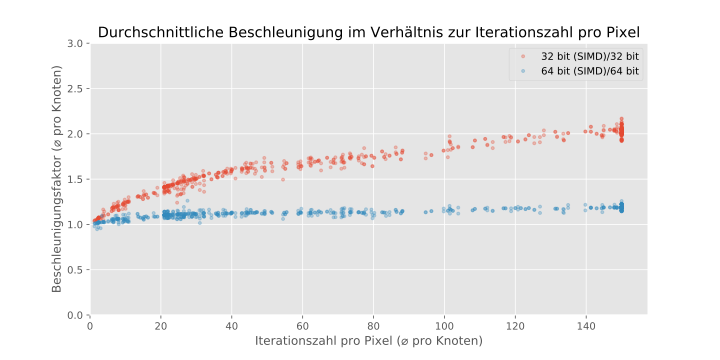
\includegraphics[width=0.9\linewidth]{img/Evaluation/simd/speedup.pdf}
	\caption{Beschleunigungsfaktor durch SIMD in Abhängigkeit von der durchschnittlichen Iterationszahl.}
	\label{fig:SIMD-speedup-vs-comptime}
\end{figure}

Zudem werden für eine Menge an Punkten stets die Zahl an Iterationen durchgeführt,
die das Maximum aller Iterationszahlen der Punkte ist.
Bei Iterationszahlen \(i_k\) des Punktvektors \(p\) ist daher
anstatt einer Rechenzeit von \(\sum_{k \in p} \frac{i_k }{ | p | }\) eine Rechenzeit von
\(\sum_{k \in p} \frac{max(i_k)_{k \in p }}{|p|} = max(i_k)_{k \in p }\) pro Punktvektor zu erwarten.
Damit wird die Beschleunigung durch SIMD kleiner, je inhomogener die Iterationszahlen sind.
Dass die Iterationszahlen im Allgemeinen am Rand der Mandelbrotmenge inhomogener sind,
wo auch die Gesamtrechenzeit geringer ist, sollte bei der Betrachtung von \autoref{fig:SIMD-speedup-vs-comptime} berücksichtigt werden.


\subsection{Lastbalancierung}
% Florian
% Wir haben zwei Klassen (naive, prediction) und wählen davon jeweils den besten 
% (naive Recursive, prediction Recursive)
Zur Lastbalancierung gibt es zwei Strategien in jeweils zwei Varianten, zur Evaluierung wird allerdings nur die rekursive Variante der beiden Strategien betrachtet.
Man stellt leicht fest, dass die nicht-rekursive Variante für Primzahlen als Worker-Anzahl schlecht ist, weil dabei nur eine Aufteilung in Zeilen oder Spalten möglich ist.
Da die Aufteilungsmöglichkeiten zusätzlich durch die Betrachtung von Tiles als atomaren Einheiten beschränkt werden, erzeugt diese Variante bereits für eine geringe Anzahl an Workern verhältnismäßig viele Leerregionen (d.h. untätige Worker).

% Erst naiver Balancer, dann prediction dafür jeweils:
% 	Plot der distribution function (Median, Max)
% 	Maximale Rechenzeit & Wie gut sind die Werte um den Median verteilt
% 	3 Plots mit Regionen außerhalb, im Rand und innerhalb der Mandelbrotmenge
Um die naive Strategie und die Strategie mit Vorhersage zu vergleichen werden drei Klassen von Regionen betrachet (vgl. \autoref{fig:testRegions}), für die es unterschiedliche Erwartungen gibt:

\begin{itemize}
	\item Regionen innerhalb der Mandelbrotmenge: Die Rechenzeiten sind bei beiden Strategien gleichmäßig hoch
	\item Regionen außerhalb der Mandelbrotmenge: Die Rechenzeiten sind bei beiden Strategien gleichmäßig niedrig
	\item Regionen am Rand der Mandelbrotmenge: Für die naive Strategie wird hier eine große Streuung der Rechenzeiten erwartet. Die Strategie mit Vorhersage sollte für eine Ballung um den Mittelwert sorgen.
\end{itemize}

Weiterhin wird erwartet, dass der Mittelwert der Rechenzeit pro Regionsklasse für die beiden Strategien gleichbleibt, da die selbe Region mit der selben Anzahl an Workern berechnet wird.
Für die folgenden Messungen wurden immer 17 Worker mit 1019 maximalen Iterationen verwendet.
Die Berechnung lief auf 17 Knoten, ein Worker musste also seinen Knoten mit dem Hostprozess teilen.

% Bilder und Stuff
% Vorhersage nie perfekt, deshalb Ausreißer nach oben/unten
% Teilweise größere/kleinere Teilregionen erstellt
In den folgenden Diagrammen wurde pro Rechenzeit aufgetragen welcher Anteil an Teilregionen genau diese Zeit benötigt hat.
Bei einer guten Lastbalancierung sollten sich die Rechenzeiten also um den Mittelwert ballen und die maximale Rechenzeit gering sein.

\begin{figure}
	\centering
	\includegraphics[width=0.9\linewidth]{img/Evaluation/balancers/balancers_border.png}
	\caption{Verteilung der Rechenzeiten für Randregionen}
	\label{fig:balancers_border}
\end{figure}

Den Unterschied zwischen naiver Strategie (rot) und Strategie mit Vorhersage (blau) sieht man besonders gut in der Verteilung für Randregionen (\autoref{fig:balancers_border}).
Die blauen Balken haben ihr Maximum in der Nähe des Mittelwerts, die roten Balken sind viel mehr über den Wertebereich verteilt.
Dass die Strategie mit Vorhersage vom Mittelwert abweicht und auch einige Ausreißer nach oben und unten hat lässt sich auf Ungenauigkeiten in der Vorhersage zurückführen, welche am Rand der Mandelbrotmenge besonders ausgeprägt sind (vgl. \autoref{par:load_balancing_prediction}).

\begin{figure}
	\centering
	\includegraphics[width=0.9\linewidth]{img/Evaluation/balancers/balancers_inside.png}
	\caption{Verteilung der Rechenzeiten für innere Regionen}
	\label{fig:balancers_inside}
\end{figure}

\begin{figure}
	\centering
	\includegraphics[width=0.9\linewidth]{img/Evaluation/balancers/balancers_outside.png}
	\caption{Verteilung der Rechenzeiten für äußere Regionen}
	\label{fig:balancers_outside}
\end{figure}

% Genauigkeit der Vorhersage vs maximale Rechenzeit für Randregionen 
% Plot: y: max comp time, balancer time  x: prediction Accuracy (Randregion)
% 	Diese "optimale" Genauigkeit wird aber bereits in allen vorherigen Evaluierungen des prediction Balancers verwendet
Bei der Strategie mit Vorhersage lässt sich die Genauigkeit der Vorhersage einstellen.
Deshalb wird hier eine Kosten-Nutzen Analyse durchgeführt.
Dazu werden für verschiedene Genauigkeiten die Verteilung der Rechenzeiten und die Dauer der Vorhersage aufgetragen.
Die Messungen fanden unter den selben Bedingungen wie die Obigen statt.

%% TODO folgenden absatz einbauen
% Probleme bei der Verwendung des Rekursiven Lastbalanierers:
% Da es stets im Diskreten eine Minimalgröße für die aufgeteilten Regionen gibt,
% kann es sein, dass eine Region für die eine hohe Last vorhergesagt wird viele Worker reserviert -
% diese jedoch nicht vollständig ausreizen kann, da die Maximalaufteilung schon erreicht wurde.
% Durch die dadurch entstehenden Leerregionen von nicht verwendbaren Workern
% kann eine suboptimale Aufteilung enstehen, schlechter noch als die des naiven rekursiven Balancierers.
%
% Dies kann abgeschwächt werden, indem eine Region stets nur soviel Workerressourcen erhält,
% wie sie maximal auslasten könnte (Fläche/Fläche minimaler Aufteilung)

\subsection{Didaktik}
% Max
% Konstanter Overhead wurde getestet,
% Lokal nicht so ein Problem. Somit würde das Programm auf superMUC seinen Zweck erfüllen.

\subsection{Zusammenfassung}
% Speedup
% Kombinationen von Unterschiedlichen Verbesserungen. als Plot.
% (Eine Klasse von Regionen)